%%%%%%%%%%%%%%%%%%%%%%%%%%%%%%%%%%%%%%%%%%%%%%%%%%%%%%%%%%%%%%%%%%%%%%%%%%%%%%%
% CAPÍTULO 4 - PROPUESTA DE DISEÑO DEL SITIO WEB DEL PROYECTO
%%%%%%%%%%%%%%%%%%%%%%%%%%%%%%%%%%%%%%%%%%%%%%%%%%%%%%%%%%%%%%%%%%%%%%%%%%%%%%%
\chapter{Propuesta de diseño del sitio web del proyecto}
\label{chap:webProp}
Tras la gestión necesaria de código que hemos creído oportuna para PyCardio. En el presente capítulo se muestra la solución web para el software desarrollado de PyCardio, donde trataremos de mostrar las partes que la componen y como han sido implementadas.

Para mostrar la web, el proceso que seguirá esta memoria es la de ir sección por sección donde enseñamos tanto el resultado como la implementación que sigue.

Antes de comenzar, debemos destacar que dicha web se ha implementado utilizando una plantilla adquirida por el equipo de la universidad y diseñada por el equipo WrapBootstrap, esta plantilla se la conoce en dicho servicio como Unify. El mapa de la propuesta que vamos a tratar es el representado por la figura \ref{fig:mapaWeb}.

\begin{figure}[h!]
    \centering
    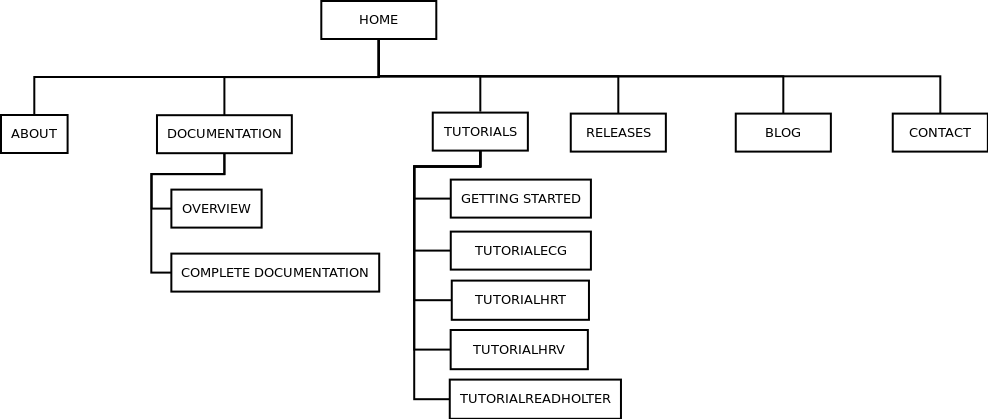
\includegraphics[width=\textwidth]{img/mapaWeb.png}
    \caption{Mapa Web de PyCardio}
    \label{fig:mapaWeb}
\end{figure}

%%%%%%%%%%%%%%%%%%%%%%%%%%%%%%%%%%%%%%%%%%%%%%%%%%%%%%%%%%%%%%%%%%%%%%%%%%%%%%%%%%%%%%%%%%
%                       HOME
%%%%%%%%%%%%%%%%%%%%%%%%%%%%%%%%%%%%%%%%%%%%%%%%%%%%%%%%%%%%%%%%%%%%%%%%%%%%%%%%%%%%%%%%%%
\section[Home]{Home \footnote{\url{https://javierfm27.github.io/}}}
\label{sec:homeWeb}
Nada más acceder en la web de PyCardio, nos encontramos en el Home de la página. El Home se ha implementado de manera que sea lo más visual y sencillo para el usuario, de modo que nada más entrar se nos ofrece la interfaz de todas las secciones, una breve descripción de qué es PyCardio, y los enlaces para redirigirnos a la documentación alojada en Read The Docs, y al código de software a la última release alojada en GitHub. \\

\begin{figure}[h!]
    \centering
    \subfloat[Captura de  Home 1]{
        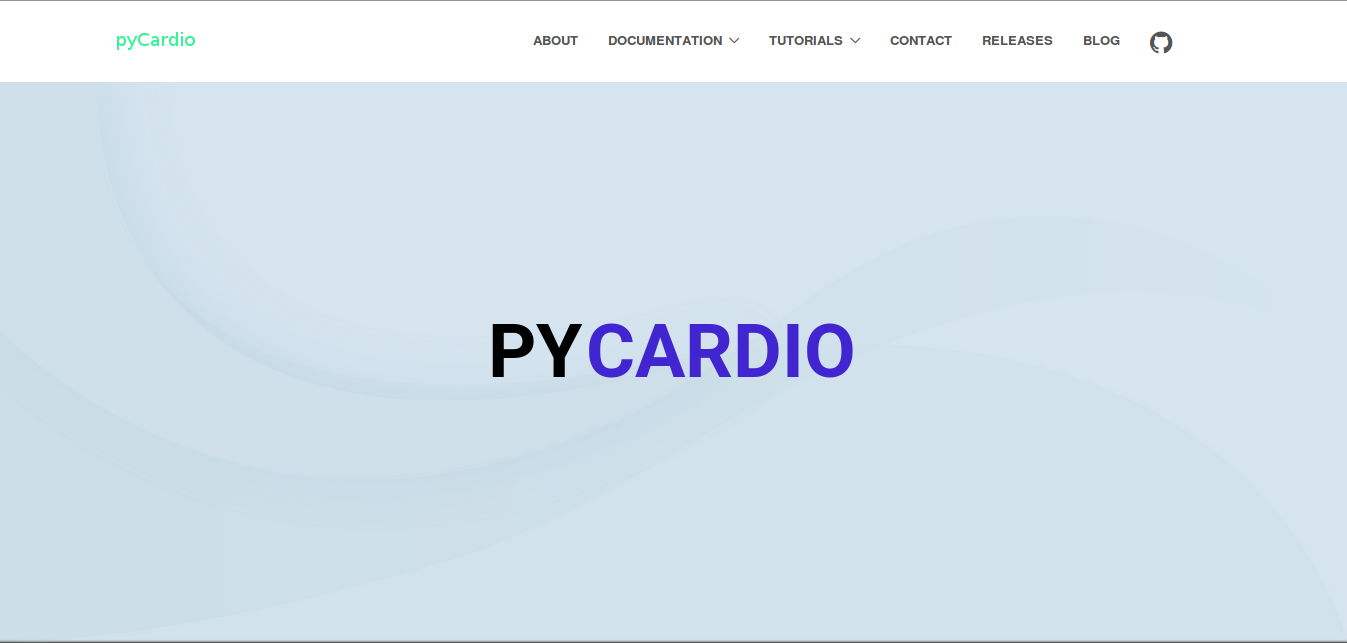
\includegraphics[width=0.8\textwidth]{img/home_1.png}
        \label{fig:home1}
    }\par
    \subfloat[Captura de Home 2]{
        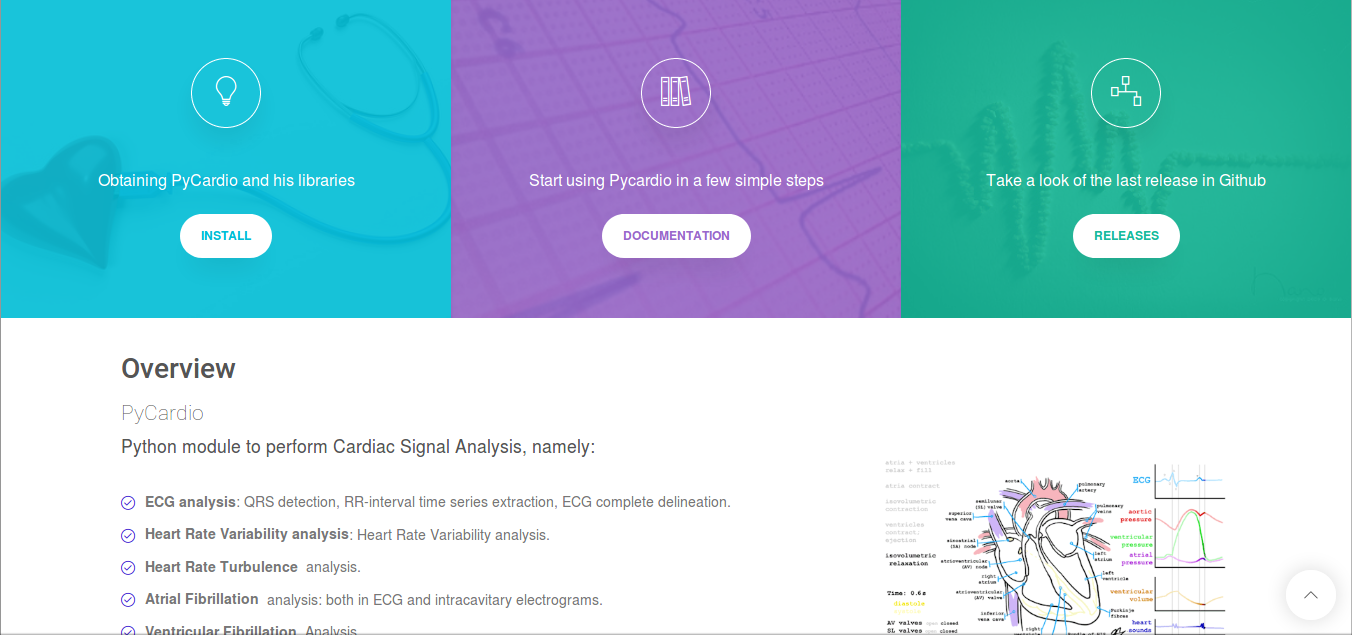
\includegraphics[width=0.8\textwidth]{img/home_2.png}
        \label{fig:home2}
    }\par
    \subfloat[Captura de Home 3]{
        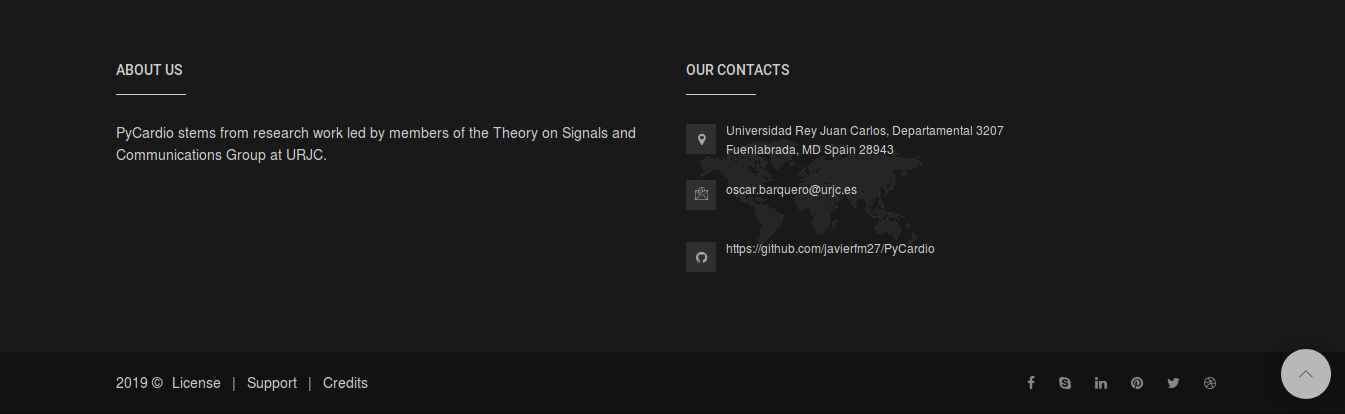
\includegraphics[width=0.8\textwidth]{img/home_3.png}
        \label{fig:home3}
    }
    \caption{Home de PyCardio}
    \label{fig:homePyCardio}
\end{figure}

Para su implementación, lo primero que se realiza es la creación de un fichero \texttt{index} en la raíz del proyecto, donde Jekyll interpretará que dicho fichero será el HTML principal de la web. El fichero puede ser escrito como ya se ha comentado, en MarkDown o en lenguaje de marcado HTML, en nuestro caso, MarkDown. El fichero solo se compone de un Front Matter en el que se llama al layout de Main, y a su vez proporciona el título de la página principal. \\



\begin{lstlisting}[language=yaml,caption=index.md. Fichero de Home de PyCardio,label=co]
    ---
layout: main
title: PyCardio Home
    ---
\end{lstlisting}

El contenido del layout main se compondrá de lenguaje HTML. Este contenido además se rellena con los mencionados \textbf{includes} en el \ref{subsec:githubJekyll}, que compondrán aquel código que se repetirá en todas las secciones de la web, permitiendo así centralizar el desarrollo de manera que, si quisiéramos cambiar el contenido de estos componentes solo tendríamos que realizar dicho cambio en un solo fichero. Para el desarrollo de este prototipo web, se han distinguido los siguientes:
\begin{itemize}
    \item \textbf{\texttt{css.html}}: En él, se incluyen todos los enlaces a los archivos CSS necesarios para la presentación final de la web.
    \item \textbf{\texttt{js.html}}: Incluye los enlaces a los archivos necesarios para el contenido de la web que hace uso de JavaScript.
    \item \textbf{\texttt{header.html}}: Contiene el panel de navegación de todas las secciones de la web.
    \item \textbf{\texttt{footer.html}}: Parte final de todas las páginas que componen la web. En ella se incluye la licencia bajo la cuál está el software, enlaces a las redes sociales del proyecto, y enlace a soporte.
    \item \textbf{\texttt{breadc.html}}: Compone el camino en el que nos encontramos dentro de la web. En él, hacemos uso del lenguaje Liquid para poder construir dicho contenido. 
\end{itemize}

Si observamos las imágenes de la figura \ref{fig:homePyCardio} podemos ver que en el layout referenciado (\texttt{ main.html})  tendremos los includes de \texttt{footer.html} y \texttt{header.html}, además de los de CSS y Javascript, estos procurarán ir en todas las páginas de la web. 

\begin{figure}[h!]
    \centering
    \subfloat[header]{
        
\includegraphics[width=\textwidth]{img/header.png}
        \label{fig:includHeader}
    }\par
    \subfloat[breadcrumber]{
        
\includegraphics[width=\textwidth]{img/breadc.png}
        \label{fig:includBread}
    }\par
    \subfloat[footer]{
        
\includegraphics[width=\textwidth]{img/footer.png}
        \label{fig:includFooter}
    }
    \caption{Includes de PyCardio}
    \label{fig:includ}
\end{figure}

El Home (página principal) de la web al ser una página única, es decir, los elementos que la componen no se repetirán en ninguna otra sección de la web, tendrá un \emph{layout} único y exclusivo solo para este uso (\texttt{main.html}). Cabe mencionar que esta plantilla también contiene los \emph{includes} de la figura \ref{fig:includ}. \\ 
Antes de pasar a tratar la siguiente sección de la web, cabe mencionar que se crea un \texttt{include} más denonminado \texttt{script.html}, que irá al final de los layouts desarrollados que contendrán aquella tecnología JQuery y Javascript que utiliza la plantilla para hacer de la web   ``sensible'', o como llamamos hoy  día a este tipo de webs \textit{responsive}.
%%%%%%%%%%%%%%%%%%%%%%%%%%%%%%%%%%%%%%%%%%%%%%%%%%%%%%%%%%%%%%%%%%%%%%%%%%%%%%%%%%%%%%%%%%
%                       ABOUT
%%%%%%%%%%%%%%%%%%%%%%%%%%%%%%%%%%%%%%%%%%%%%%%%%%%%%%%%%%%%%%%%%%%%%%%%%%%%%%%%%%%%%%%%%%
\section[About]{About \footnote{\url{https://javierfm27.github.io/about/}}}
\label{sec:aboutWeb}
Esta sección (About\footnote{\url{https://javierfm27.github.io/about/}}) de la web trata de dar una vista general de todos aquellos que han formado parte del proyecto PyCardio, tanto para su parte de desarrollo de software como en la parte de implementación de la web. 

\begin{figure}[H]
    \centering
    \subfloat[Captura de  About 1]{
        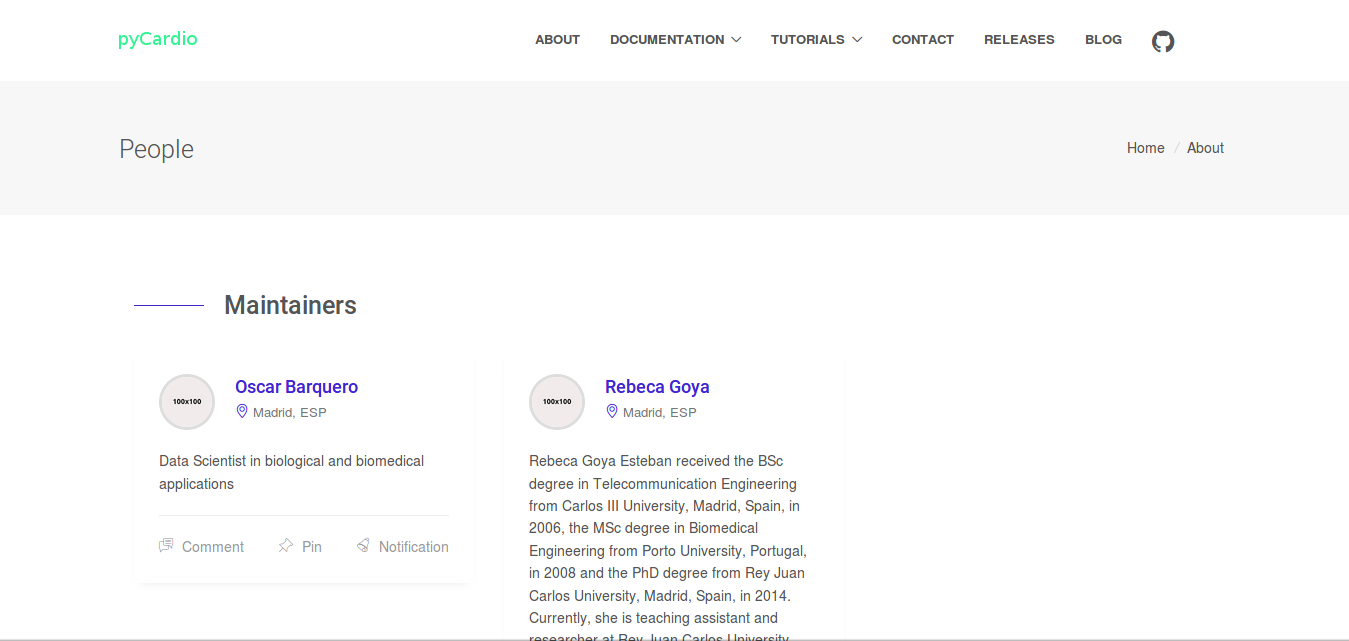
\includegraphics[width=0.5\textwidth]{img/about_1.png}
        \label{fig:aboutWeb1}
    }
    \subfloat[Captura de About 2]{
        
\includegraphics[width=0.5\textwidth]{img/about_2.png}
        \label{fig:aboutWeb2}
    }
    \caption{Sección About de la web PyCardio}
    \label{fig:aboutWeb}
\end{figure}

Para llevar a cabo esta sección, se ha diseñado un nuevo layout denominado \texttt{page.html} cuyo código es mostrado en el listing \ref{code:layoutPage}, que será utilizado para la mayoría de las páginas que se quieran añadir a la web. Tanto Jekyll en su documentación como nosotros, hacemos la siguiente distinción entre estos dos tipos de páginas:

\begin{itemize}
    \item \textbf{Pages: } Contenido que no está basado en una fecha.
    \item \textbf{Posts: } Aquel contenido que se caracteriza por la fecha en la que se publicó en la web, típicamente una entrada en un blog del sitio web.
\end{itemize}


Si observamos la plantilla mencionada, percibimos que para el desarrollo de \textit{About} usamos una variable nueva dónde el contenido se incrustará en  dicha variable del lenguaje de plantilla Liquid denominada \texttt{content}. Al incluir \textit{shortcodes}\footnote{Fragmentos de código utilizadas por los plugins que en este caso se adjuntan con la plantilla Unify adquirida.} de la plantilla Unify el contenido que tendrá nuestro fichero principal de la sección \textit{about} será HTML.

El \textit{shortcode} empleado trata de un elemento de bloque en el que solo se hace uso de los CSS en conjunción con la plantilla. Quedando así tal y como lo muestra el listing \ref{code:about}. \\

Antes de continuar probablemente os hayáis preguntado el porqué de otro fichero \texttt{index} si ya habíamos diseñado uno para el Home de nuestra web. Pues bien,  cuando tenemos varias páginas en nuestra página web, lo más eficaz es seguir un orden en los directorios. Por lo tanto si estamos desarrollando la sección \texttt{about}, tengamos en un directorio \texttt{/about/}, todos aquellos contenidos que compondrán esta sección. De manera que, para Jekyll, el fichero en el directorio \texttt{/about/index.html}, será el fichero principal para esa sección.

Así si escribimos un hiperenlace en nuestro web escribiendo \texttt{\{\{site.url\}\}/about/} \footnote{\texttt{\{\{site.url\}\}} es una variable del \textit{framework} Jekyll definido en el fichero de configuración(\texttt{config.yml}) donde obtenemos la dirección URL del sitio web}, nos mostrará el contenido generado por \texttt{index.html} en nuestro directorio \texttt{/about/}.

Cabe destacar la introducción de un nuevo elemento en el \textit{layout} del que se hace referencia en esta sección, haciendo uso del \textit{include} de \texttt{breadc.html} y utilizando la variable \texttt{page}, que brinda información de página específica, permitiendo el uso de las variables definidas en el Front Matter, y de setencias de control del lenguaje de plantilla Liquid,  diferenciándole del mencionado con anterioridad. 

\begin{lstlisting}[style=htmlcssjs,caption=Breadcrumber,label={code:breadcrum}]
  <div class="align-self-center ml-auto">
          <ul class="u-list-inline">
            <li class="list-inline-item g-mr-5">
              <a class="u-link-v5 g-color-main" href="{{site.url}}">Home</a>
              <i class="g-color-gray-light-v2 g-ml-5">/</i>
            </li>
            
            
            

               
                
                  <li class="list-inline-item g-mr-5">
                  {{page.title}}
                  </li>
                
              
                <li class="list-inline-item g-mr-5">
                  <a class="u-link-v5 g-color-main">{{ element |capitalize }}</a>
                  

                  
                    <i class="g-color-gray-light-v2 g-ml-5">/</i>
                  
                </li>
              

            
          </ul>
        </div>
\end{lstlisting}

En este caso el uso que hacemos de la información es el dado por \texttt{\{\{page.path\}\}} y de \texttt{\{\{page.title\}\}} donde accedemos al directorio y título del archivo que hace uso de en este caso, de \texttt{breadc.html}.

%%%%%%%%%%%%%%%%%%%%%%%%%%%%%%%%%%%%%%%%%%%%%%%%%%%%%%%%%%%%%%%%%%%%%%%%%%%%%%%%%%%%%%%%%%
%                       DOCUMENTATION
%%%%%%%%%%%%%%%%%%%%%%%%%%%%%%%%%%%%%%%%%%%%%%%%%%%%%%%%%%%%%%%%%%%%%%%%%%%%%%%%%%%%%%%%%%
\section[Documentation]{Documentation \footnote{\url{https://javierfm27.github.io/documentation/overview.html}}}
\label{sec:docWeb}

Apartado donde se da a conocer el software desarrollado, para ello esta sección se divide en dos, donde por una parte se trata el paquete con una perspectiva general de su utilidad, de lo que trata y de los módulos que lo componen y por otro lado se da a conocer de todas las funciones que componen PyCardio, es decir, la documentación de funciones, módulos, y clases del software.

\begin{figure}[h!]
    \centering
    \subfloat[Sección Overview]{
        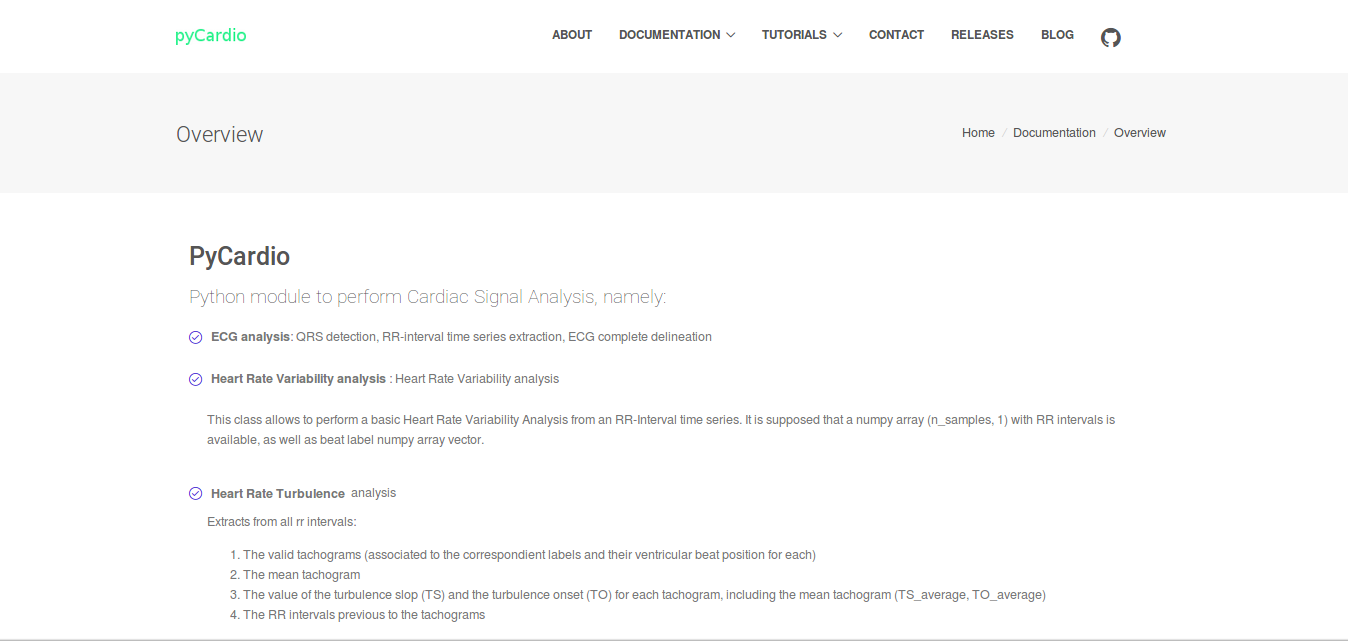
\includegraphics[width=0.5\textwidth]{img/doc_1.png}
        \label{fig:docWeb1}
    }
    \subfloat[Sección Complete Documentation]{
        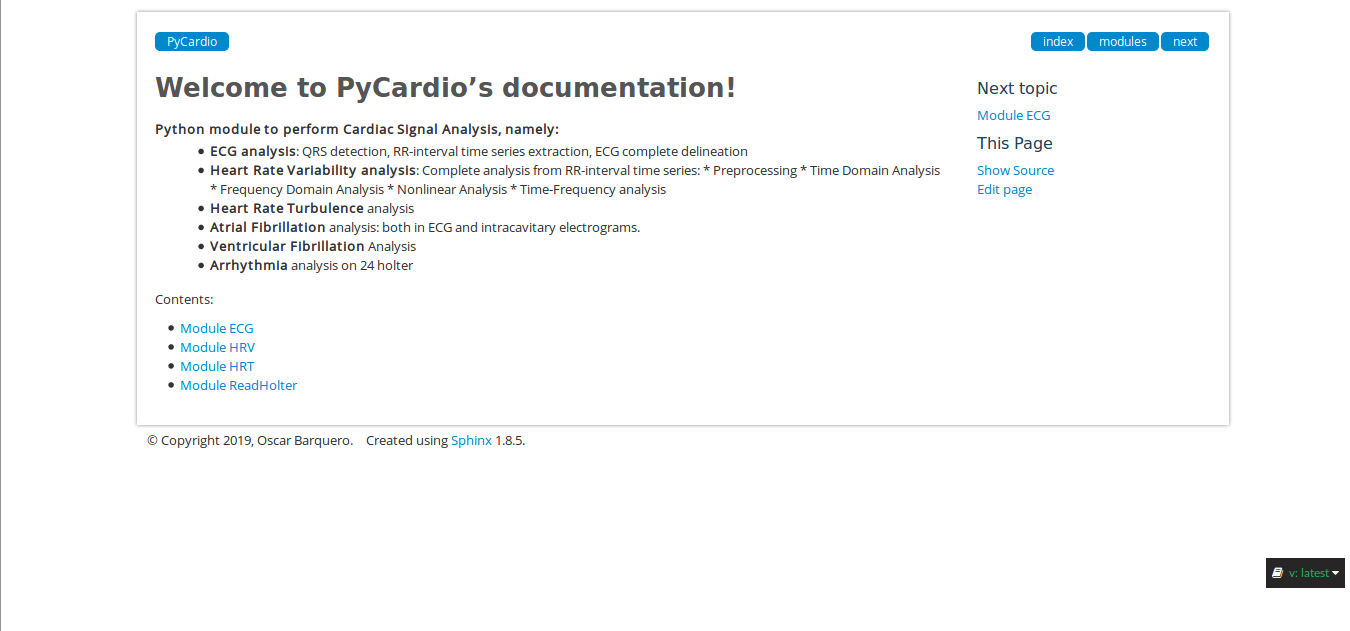
\includegraphics[width=0.5\textwidth]{img/doc_2.png}
        \label{fig:docWeb2}
    }
    \caption{Sección Documentation de la web PyCardio}
    \label{fig:docWeb}
\end{figure}


Para la implementación del contenido que se muestra en la figura \ref{fig:docWeb1} hemos usado la plantilla definida de \texttt{page.html}, por tanto, para su desarrollo lo único que ha hecho falta es escribir el contenido que esta contendrá en HTML. Como ya sabemos, la página mostrada en la figura \ref{fig:docWeb2} es la que se ha implementado en el capítulo \ref{chap:codeManagement} con la tecnología Read The Docs.
%%%%%%%%%%%%%%%%%%%%%%%%%%%%%%%%%%%%%%%%%%%%%%%%%%%%%%%%%%%%%%%%%%%%%%%%%%%%%%%%%%%%%%%%%%
%                       TUTORIALS
%%%%%%%%%%%%%%%%%%%%%%%%%%%%%%%%%%%%%%%%%%%%%%%%%%%%%%%%%%%%%%%%%%%%%%%%%%%%%%%%%%%%%%%%%%
\section{Tutorials}
\label{sec:tutoWeb}

Parte de la web centrada  tanto en dar un guión de como empezar a usar el paquete PyCardio como en mostrar un ejemplo de uso para cada módulo que compone el software. Para ello se divide en cinco apartados, uno por cada módulo y uno exclusivo para mostrar como empezar a aplicar PyCardio a nuestros desarrollos.

Antes de mostrar el contenido de este apartado es de mencionar que está incompleto debido a que el paquete sigue en fase beta y por tanto la parte de información de como usar sus módulos también. Por ello, se ha implementado el contenido de la parte que muestra como usarlo, y el tutorial del módulo HRV. 

\begin{figure}[h!]
    \centering
    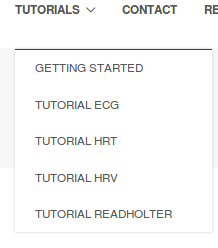
\includegraphics[width=0.5\textwidth]{img/tutorials_panel.png}
    \caption{Secciones de Tutorials }
    \label{fig:tutoWebPanel}
\end{figure}





\subsection[Getting Started]{Getting Started \footnote{\url{https://javierfm27.github.io/tutorials/getting_started.html}}}
El contenido web de esta subsección de \textit{tutorials} se centra en enseñar como instalar el paquete y como aplicarlo. Al no disponer de la información de como usar el paquete, se ha procedido a implementar una plantilla para su uso futuro cuando se disponga de mas información. En dicha plantilla podemos distinguir trozos de inserción de código, gráficas y texto. 

\begin{figure}[h!]
    \centering
    \subfloat[Captura de  Getting Started 1]{
        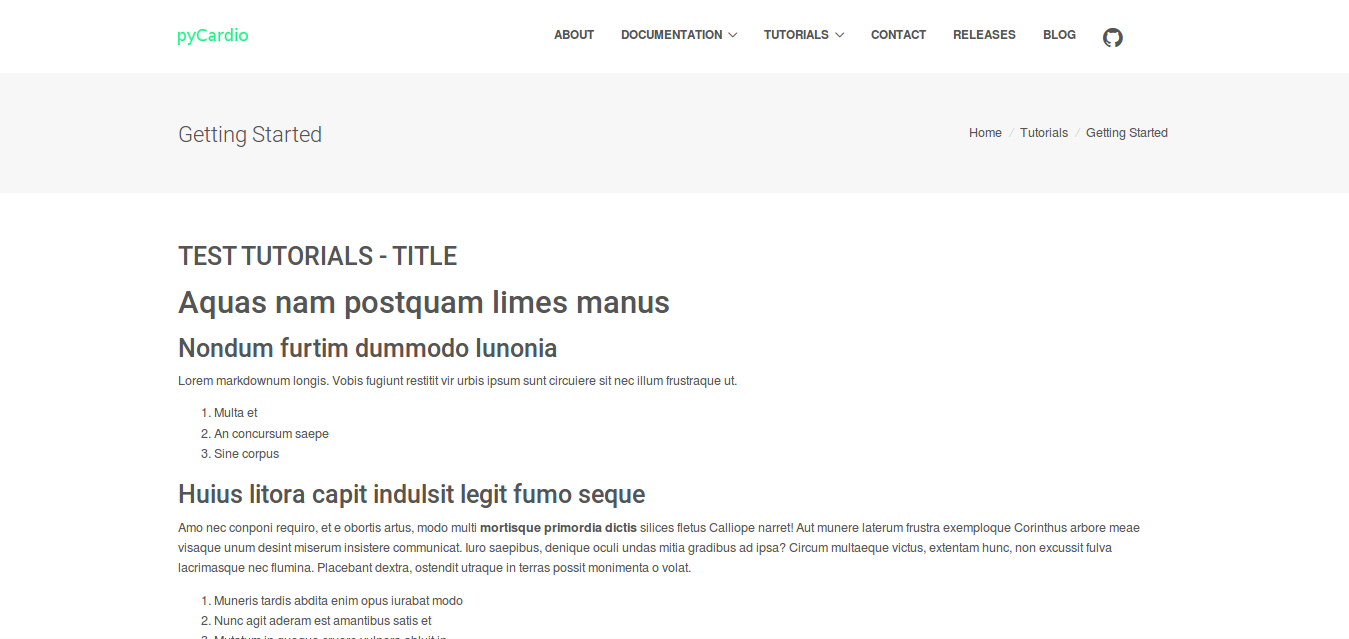
\includegraphics[width=0.7\textwidth]{img/gettin_1.png}
        \label{fig:gettinWeb1}
    }\par
    \subfloat[Captura de  Getting Started 2]{
        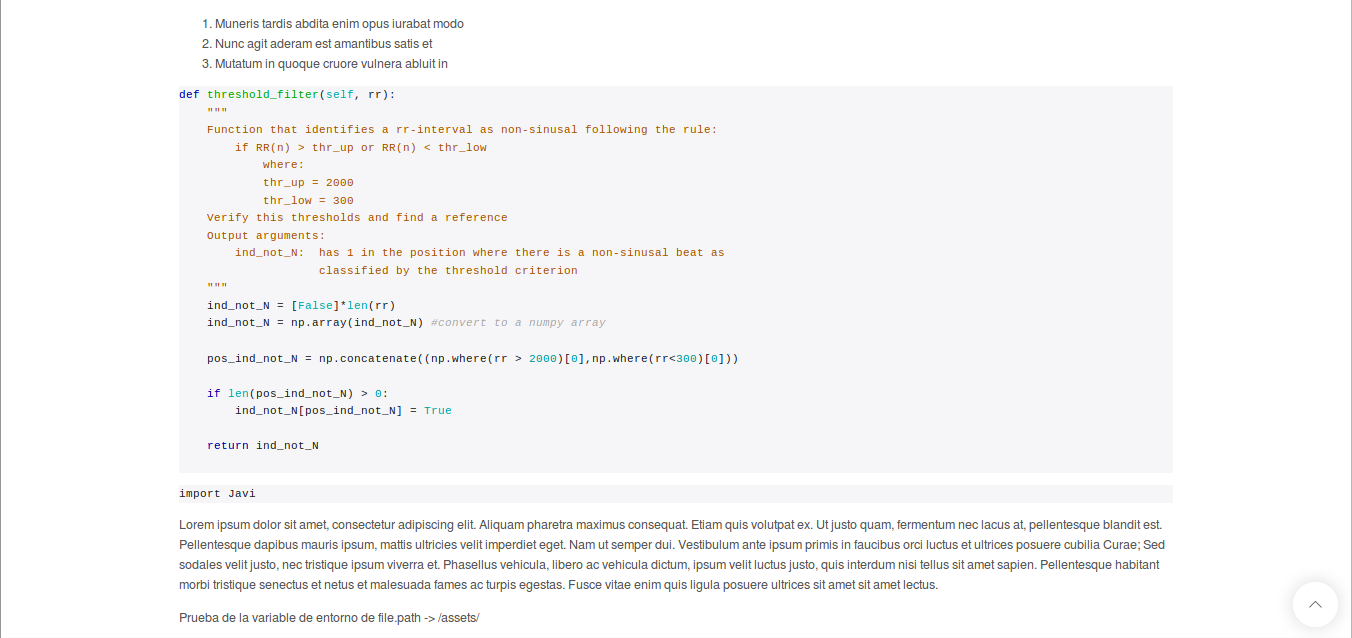
\includegraphics[width=0.7\textwidth]{img/gettin_2.png}
        \label{fig:gettinWeb2}
    }\par
    \subfloat[Captura de  Getting Started 3]{
        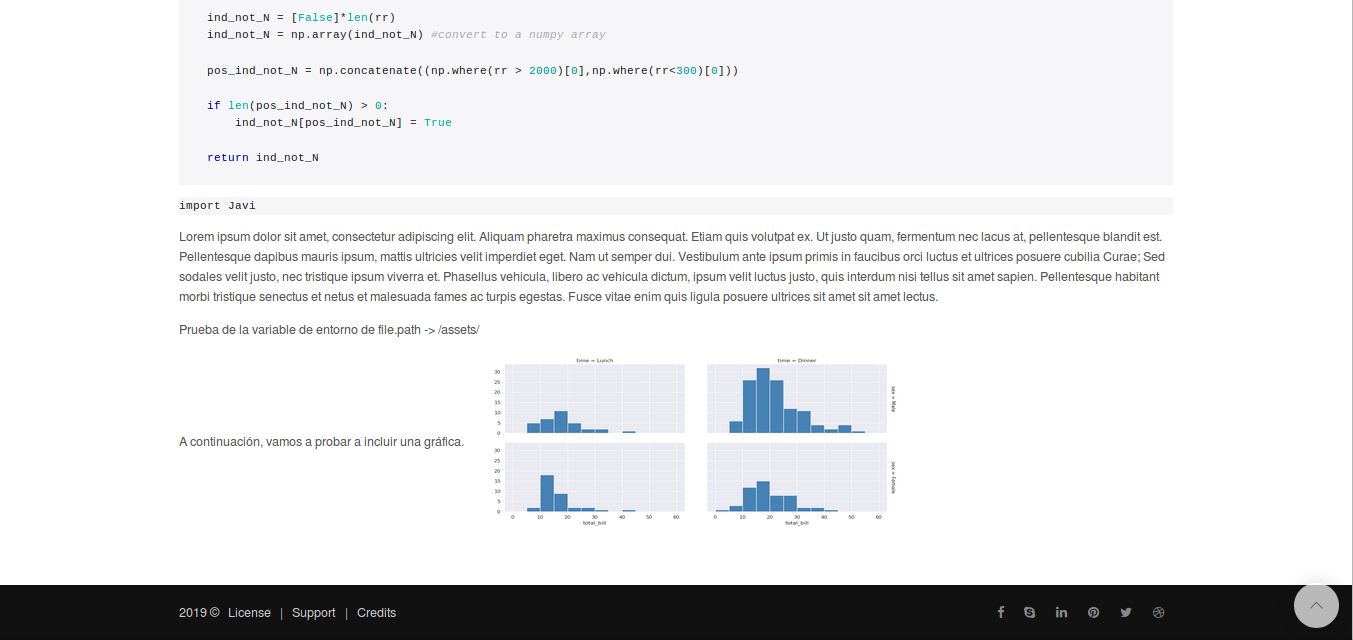
\includegraphics[width=0.7\textwidth]{img/gettin_3.png}
        \label{fig:gettinWeb3}
    }
    \caption{Subsección Getting Started de Tutorials }
    \label{fig:gettinWeb}
\end{figure}

Su implementación a diferencia de lo demás visto hasta ahora esta escrita en MarkDown. Para ello, como venimos haciendo, en el Front Matter de nuestro fichero damos un título y referenciamos el layout que se va a usar para mostar el contenido escrito. \\

Si observamos las  últimas líneas del Listing \ref{code:gettingMark} podemos ver que también es posible escribir HTML en nuestro contenido, aunque el archivo sea de tipo MarkDown.

\subsection[Tutorial HRV]{Tutorial HRV \footnote{\url{https://javierfm27.github.io/tutorials/hrv.html}}}
Tomando la plantilla escrita para la sección de \textit{getting started} en la que insertamos gráficas, código y escribimos texto plano se ha implementado la sección de tutorial HRV usando la información que se ha proporcionado por los creadores de \textit{PyCardio} a través de un \textit{jupyter notebook}\footnote{Entorno de trabajo interactivo que permite desarrollar en código Python.} pudiendo así mostrar en la web una guía de como utilizar este módulo. 


\begin{figure}[h!]
    \centering
    \subfloat[Captura de HRV 1]{
        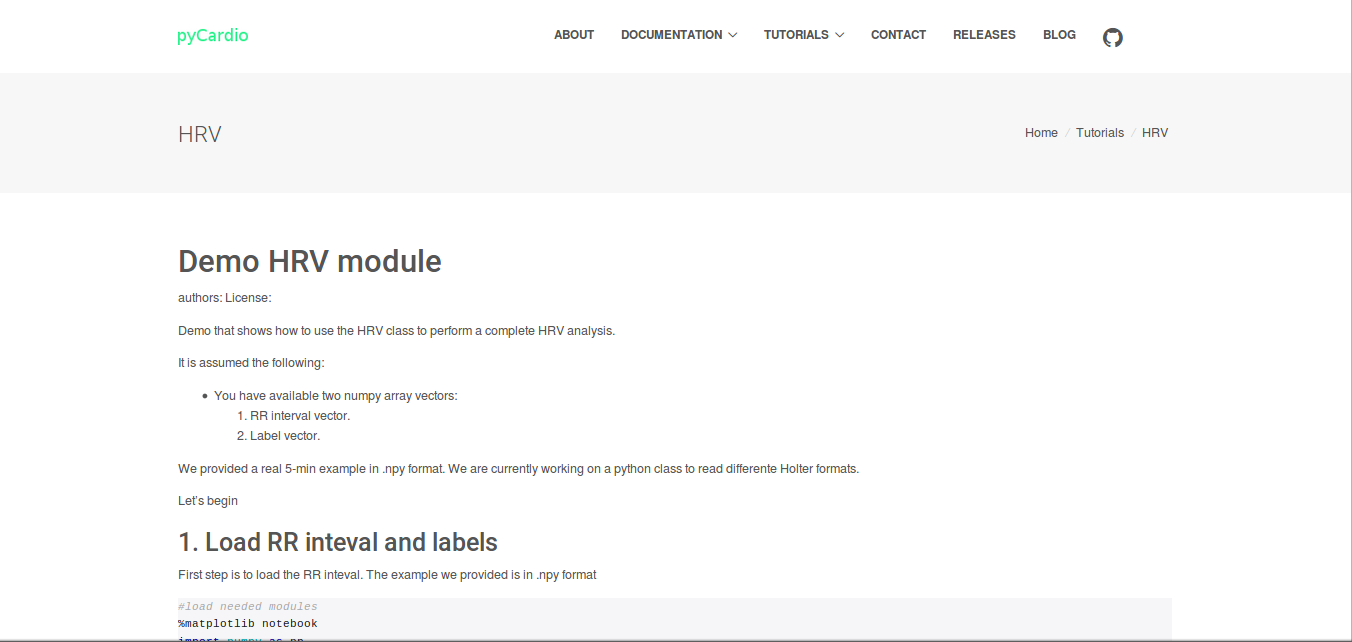
\includegraphics[width=0.7\textwidth]{img/hrv_1.png}
        \label{fig:hrvWeb1}
    }\par
    \subfloat[Captura de HRV 2]{
        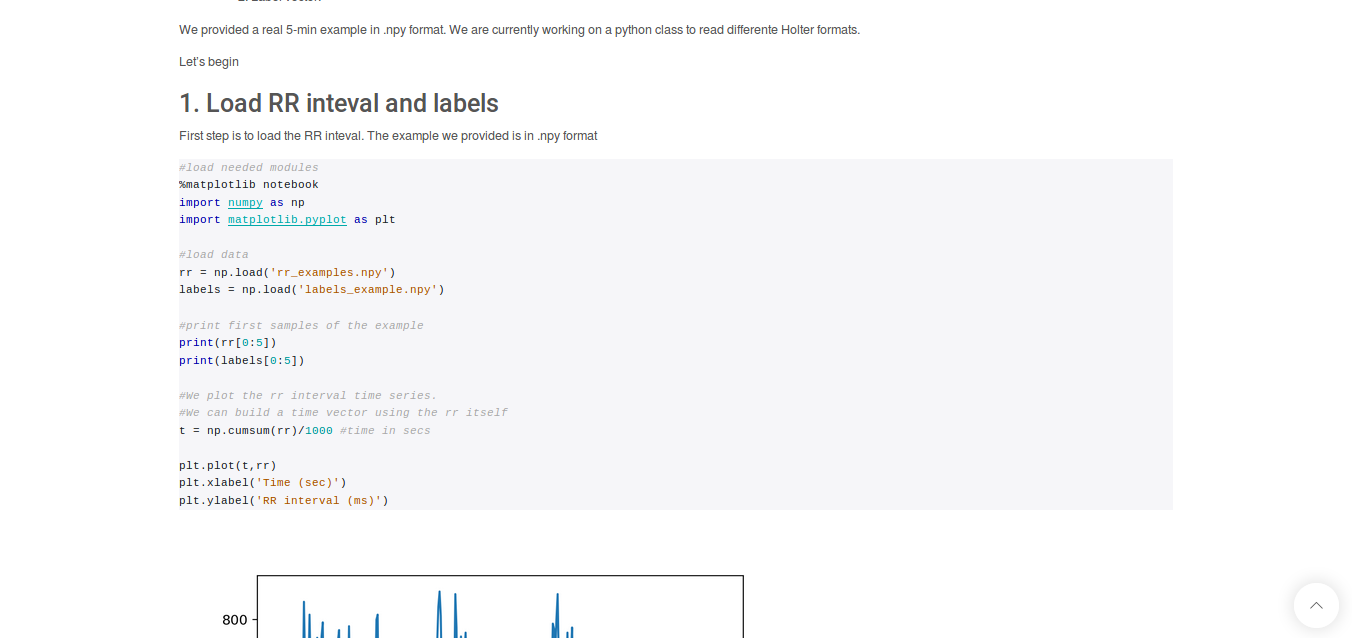
\includegraphics[width=0.7\textwidth]{img/hrv_2.png}
        \label{fig:hrvWeb2}
    }\par
    \subfloat[Captura de HRV 3]{
        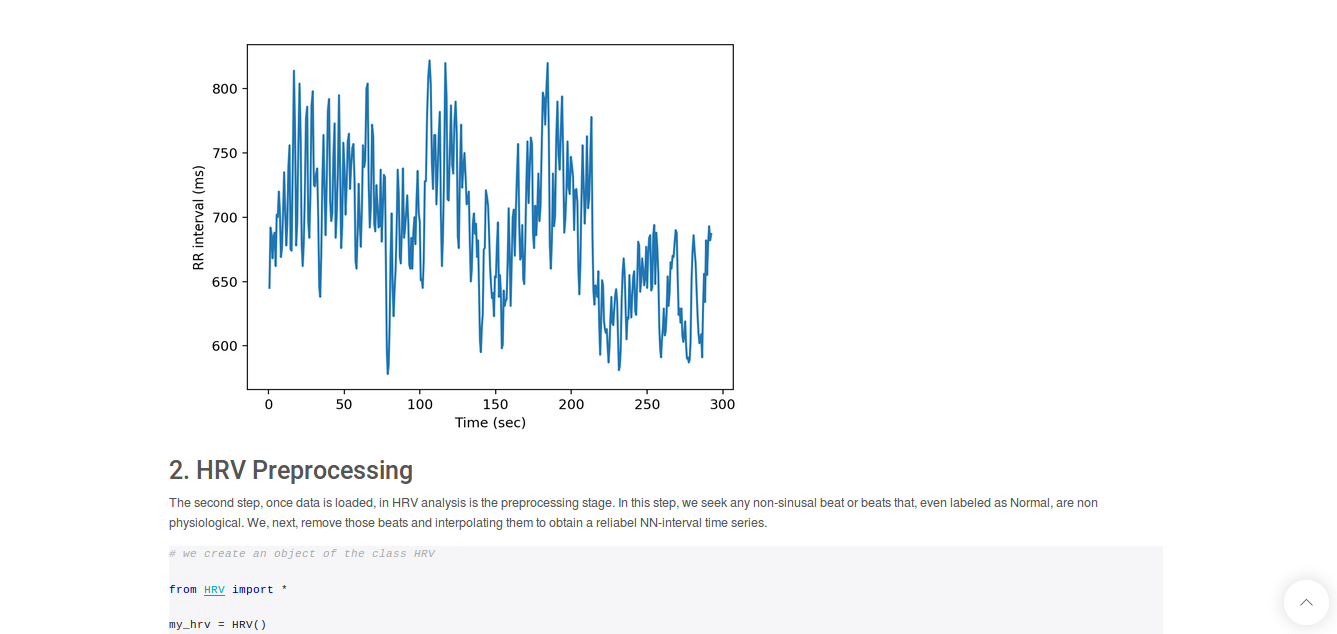
\includegraphics[width=0.7\textwidth]{img/hrv_3.png}
        \label{fig:hrvWeb3}
    }
    \caption{Subsección HRV de Tutorials}
    \label{fig:hrvWeb}
\end{figure}

Si examinamos las capturas realizadas de la sección en la figura \ref{fig:hrvWeb} tenemos un ejemplo de lo comentado anteriormente, texto plano, gráficas e inserción de código. Además de cambiar el tipo de fuente cuando insertamos código, comprobamos cómo dependiendo de las palabras reservadas utilizadas en el lenguaje especifico estas están resaltadas de una manera u otra. Para llevar a cabo el resaltado de código se ha utilizado un resaltador escrito en  \textit{Ruby} denominado \textit{Rouge}, se hace posible su uso añadiendo al fichero de configuración la setencia \texttt{higlighter: rouge}.

%%%%%%%%%%%%%%%%%%%%%%%%%%%%%%%%%%%%%%%%%%%%%%%%%%%%%%%%%%%%%%%%%%%%%%%%%%%%%%%%%%%%%%%%%%
%                       CONTACT
%%%%%%%%%%%%%%%%%%%%%%%%%%%%%%%%%%%%%%%%%%%%%%%%%%%%%%%%%%%%%%%%%%%%%%%%%%%%%%%%%%%%%%%%%%

\section[Contact]{Contact \footnote{\url{https://javierfm27.github.io/contact/}}}
\label{sec:contactWeb}
Contenido web centrado en mostrar quién es el autor del paquete \textit{PyCardio} dando información de trayectoria, dedicación y proyectos en los que ha colaborado o autorizado. Además, se incluye un formulario con la intención de sugerir dudas, inscribirse al blog de la web y así como recibir información de futuras \textit{releases}.

\begin{figure}[H]
    \centering
    \subfloat[Captura de  Contact 1]{
        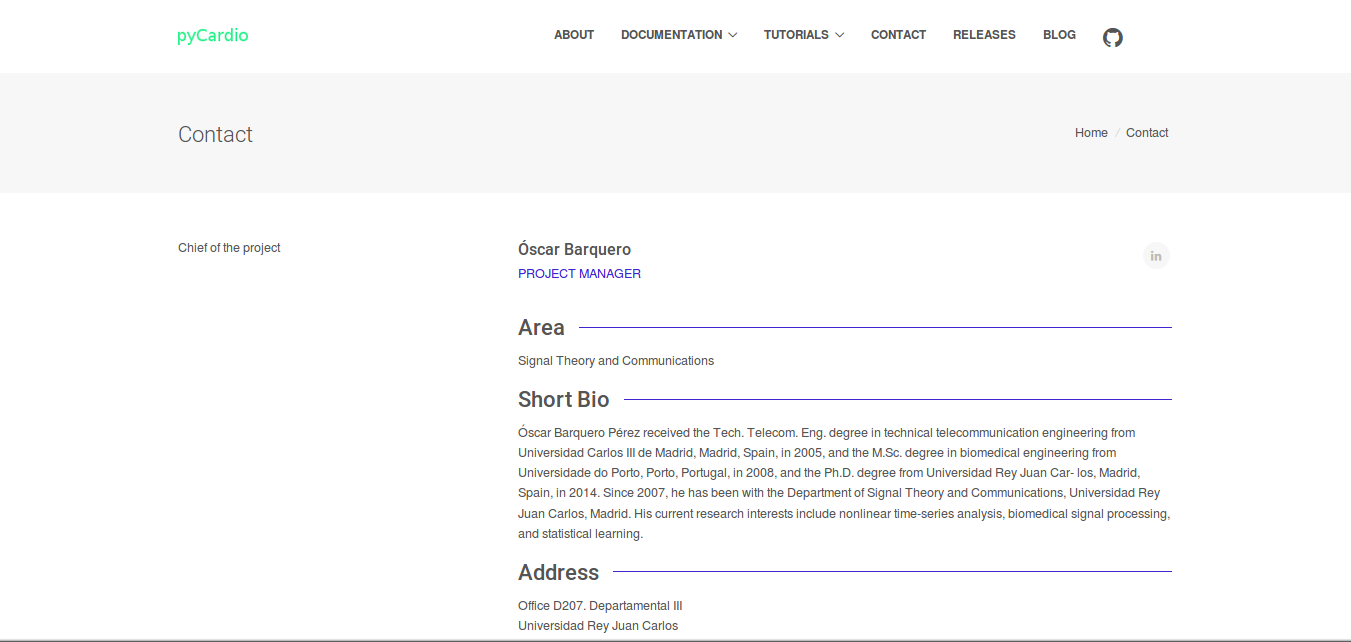
\includegraphics[width=0.4\textwidth]{img/contact_1.png}
        \label{fig:contactWeb1}
    }
    \subfloat[Captura de Contact 2]{
        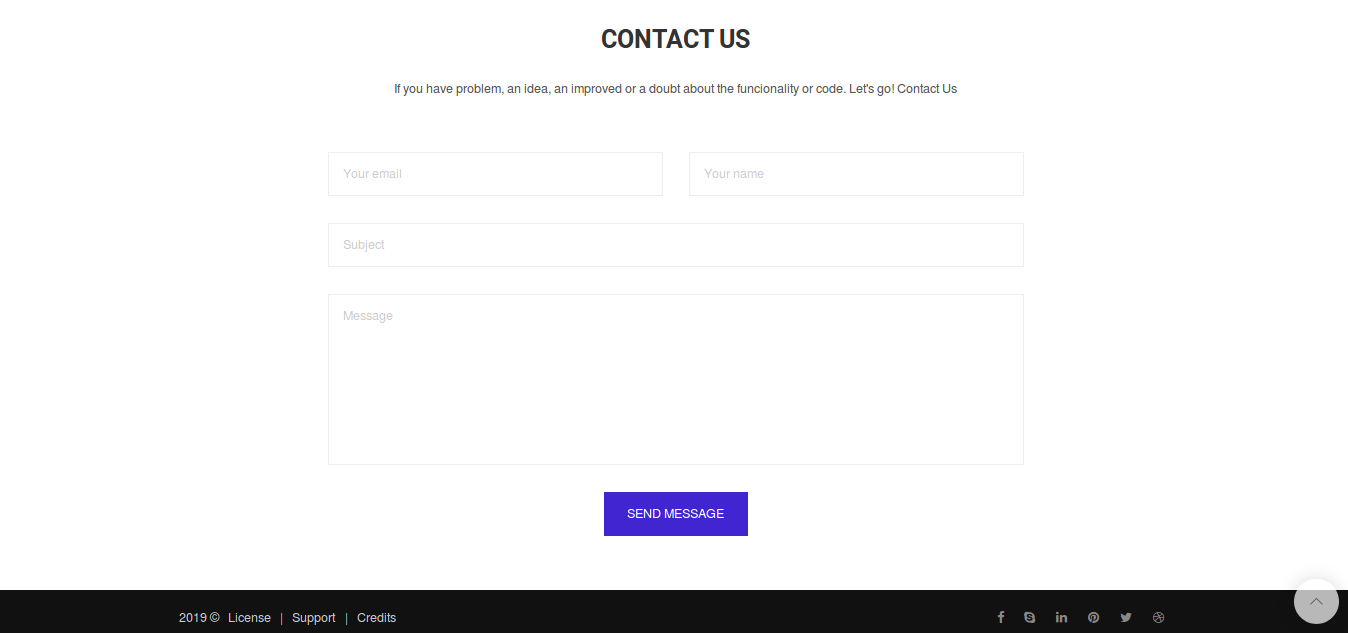
\includegraphics[width=0.4\textwidth]{img/contact_2.png}
        \label{fig:contactWeb2}
    }
    \caption{Sección Contact de la Web}
    \label{fig:contactWeb}
\end{figure}


La parte que consiste en proporcionar la información del autor se ha desarrollado como se ha ido realizando hasta ahora, creando un fichero \texttt{index.html} en el directorio \texttt{/contact/} que utilizará el \textit{layout Page}. Tanto la parte visual (CSS) y contenido (HTML) de toda la sección se ha diseñado usando el abanico de \textit{shortcodes} proporcionados por la plantilla \textit{Unify}. \\

Contemplando la figura  \ref{fig:contactWeb2} vemos que el formulario que se basa en contactar con los desarrolladores se compone de diversos campos. Toda la información recogida en estos compondrán un \textit{email} que será enviado al correo de los autores de \textit{PyCardio}. Para implementar esta parte se ha hecho uso de una API de \textit{JavaScript} que envía correo directamente desde su código en la web. El servicio utilizado es \textit{emailJs}\footnote{\url{https://www.emailjs.com/}}

El uso de este servicio se ha realizado siguiendo estos pasos:
\begin{enumerate}
    \item Nos registramos con una cuenta, al ser el primer registro se proporciona una cuota de 200 \textit{emails} gratis. Tras ellos, es necesario desembolsar una cuota mensual.
    \item Se crea una plantilla con la finalidad de completarla con lo obtenido en el formulario mediante \textit{JQuery}.
    \item Implementación de código \textit{JavaScript} y \textit{JQuery} encargado de obtener la información y finalmente enviar el correo.
\end{enumerate}

\begin{figure}[H]
    \centering
    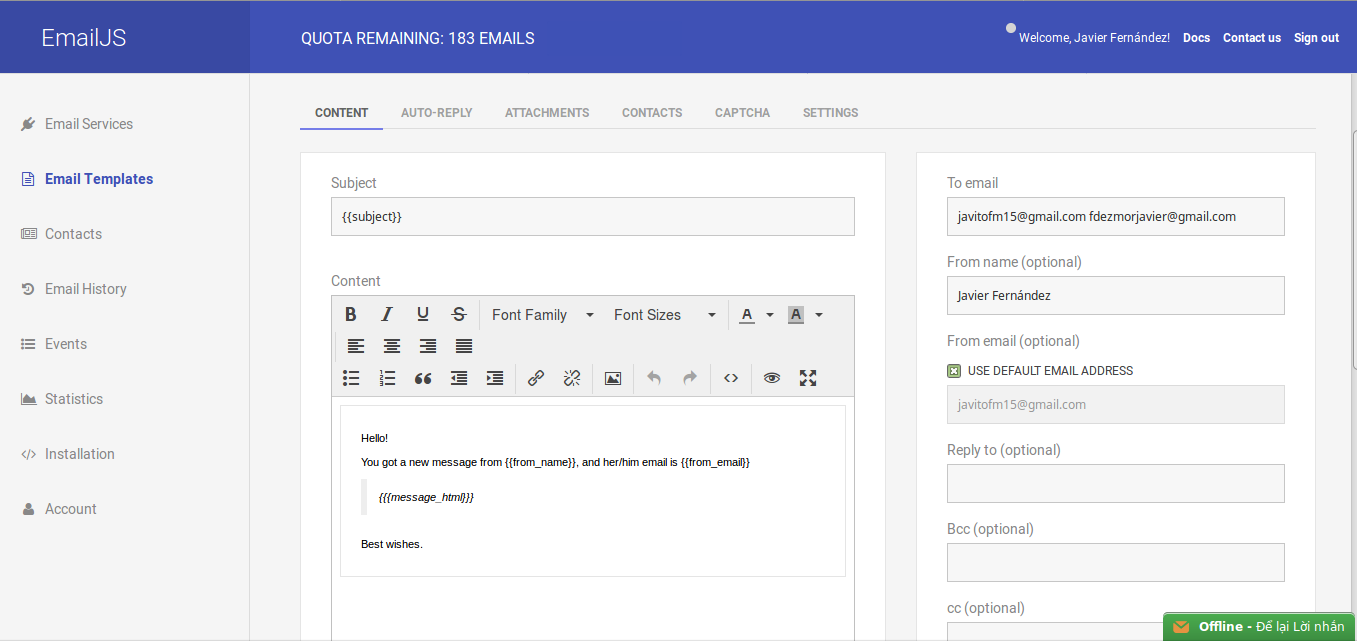
\includegraphics[width=\textwidth]{img/email_template.png}
    \caption{Plantilla \textit{email}}
    \label{fig:emailTemplate}
\end{figure}

Exceptuando el paso de registro, que solo trata de obtener una cuenta válida para el uso del servicio, vamos a explicar el proceso seguido para los otros. 

\subsubsection*{Creación de plantilla de correo}
Este paso se realiza a través de la interfaz gráfica que proporciona el servicio \textit{emailJS} que únicamente consiste en definir la forma que obtendrá el contenido del correo que llegará a los destinatarios que elijamos. Este contenido aparte de obtener texto también se establece mediante las variables de plantilla. Si observamos la plantilla definida en la figura \ref{fig:emailTemplate} vemos que tenemos las siguientes variables para nuestro contenido personalizado:
\begin{itemize}
    \item \{\{$subject$\}\}: Asunto del correo.
    \item \{\{$from\_name$\}\}: Nombre del sugerente recogido en la web. 
    \item \{\{$from\_email$\}\}: \textit{Email} de la persona que solicita o envía información a través del formulario.
    \item \{\{$message\_html$\}\}: Contenido del mensaje que es escrito por el usuario de la web.
\end{itemize}

\subsubsection*{Código \textit{JQuery} y \textit{JavaScript}}
Ya tenemos la cuenta y la plantilla, por tanto, solo nos queda obtener la información. El código que se encargará de dicha acción se incluirá al final del contenido HTML en un elemento \texttt{script}. Podemos así separar dos secciones de código dentro del \textit{script}, una parte encargada de recoger la información y otra, cuya meta es enviar el correo usando el servicio \textit{emailJS}.

La obtención se realiza con el evento de \textit{JQuery} \texttt{focusout()} que se ejecuta cuando cambiamos de campo en la web. Un ejemplo de esto sería el dado por el Listing \ref{code:jquery1}, que como vemos asignamos a la variable \texttt{$template\_params.message\_html$} lo escrito en el formulario de clase \texttt{message-form}. La tupla de valores \texttt{$template\_params$} contendrá todos las varibles de plantilla y su contenido. 

\begin{lstlisting}[caption=Código para obtener la información de \texttt{message-form},label={code:jquery1}]
  $(".message-form").focusout(function() {
    template_params.message_html = $(this).val();
  });
\end{lstlisting}

Tras agrupar toda la información en nuestra variable, sólo nos queda hacer posible el envío del correo. Para ese fin, antes de ejecutar la función del servicio \texttt{emailjs.send()} pasando por parámetro el servicio utilizado, la plantilla, y los valores de la variables, debemos habilitar el uso de la interfaz, que se consigue, incluyendo el código mostrado en el Listing \ref{code:initEmailJS}, el valor que se pasa por parámetro a la función \texttt{emailjs.init()} es el API \textit{key} asociado al usuario. Para que funcione la aplicación el código mencionado debe ir en la cabecera \textit{head} de la página que vaya a utilizarla

\begin{lstlisting}[caption=Código que permite conectarse con la interfaz de \textit{emailJs},label={code:initEmailJS}]
  <!-- EMAILJS -->
<script type="text/javascript" src="https://cdn.emailjs.com/sdk/2.3.2/email.min.js"></script>
<script type="text/javascript">
   (function(){
      emailjs.init("user_Hopd6SgEyxvsIFC4VTcCc");
   })();
</script>
\end{lstlisting}


Una vez que se inicia la conexión para manejar \textit{emailJS}, hacemos uso de la función \texttt{send()} de igual manera que la mostrada en el Listing \ref{code:sendEmail} , donde vemos que las sentencias se ejecutan a partir de cuando se produce el evento \textit{JQuery} \texttt{click} en el bóton que compone el final del formulario.

\begin{lstlisting}[caption=Código que produce el envío de correo,label={code:sendEmail}]
  $("#enviarEmail").click(function() {
    var service_id = "default_service";
    var template_id = "template_SDZsLF1w";
    emailjs.send(service_id, template_id, template_params)
      .then(function(response) {
        alert('SUCCESS!', response.status, response.text);
      }, function(error) {
        alert('FAILED...', error);
      });
    alert("Email Send!");
  });
\end{lstlisting}

Un ejemplo de lo conseguido por estos tres pasos es el mostrado en la figura \ref{fig:sendEmail}.

\begin{figure}[H]
    \centering
    \subfloat[Formulario \textit{Web}]{
        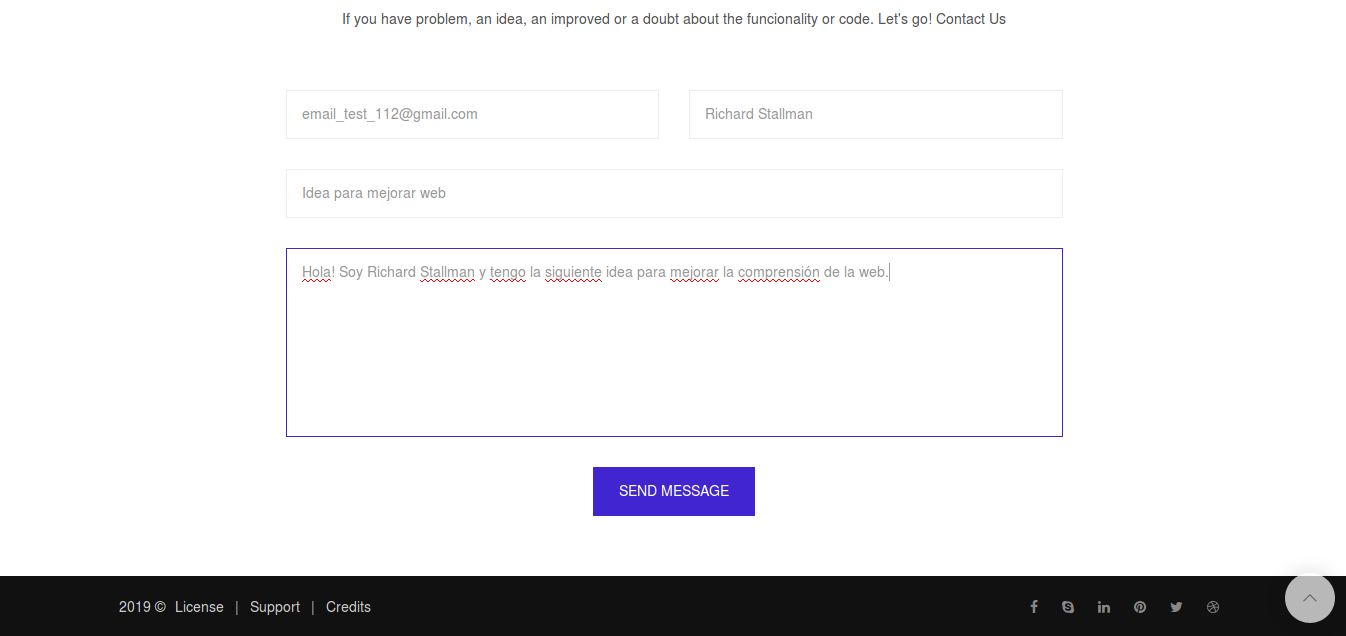
\includegraphics[width=0.5\textwidth]{img/send_email_1.png}
        \label{fig:sendEmail1}
    }
    \subfloat[Correo Recibido]{
        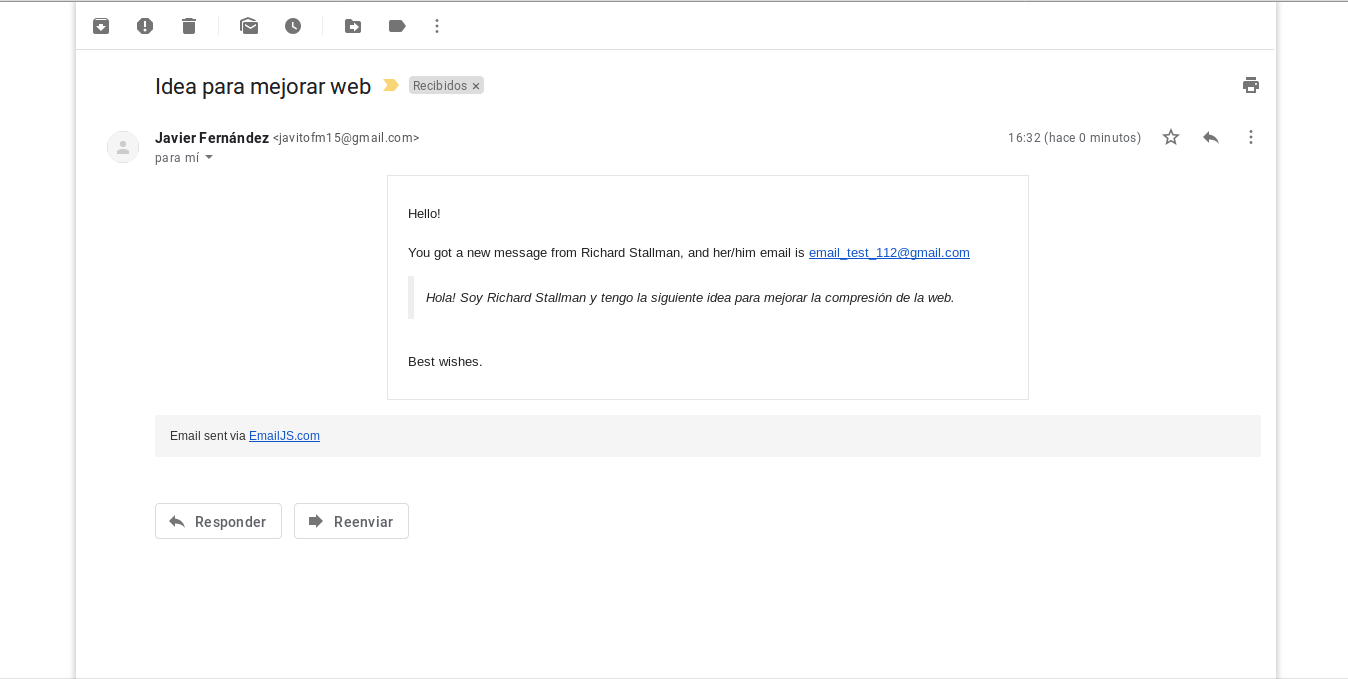
\includegraphics[width=0.5\textwidth]{img/send_email_2.png}
        \label{fig:sendEmail2}
    }
    \caption{Ejemplo sencillo de envío de correo en \textit{PyCardio Web}}
    \label{fig:sendEmail}
\end{figure}

%%%%%%%%%%%%%%%%%%%%%%%%%%%%%%%%%%%%%%%%%%%%%%%%%%%%%%%%%%%%%%%%%%%%%%%%%%%%%%%%%%%%%%%%%%
%                       RELEASE
%%%%%%%%%%%%%%%%%%%%%%%%%%%%%%%%%%%%%%%%%%%%%%%%%%%%%%%%%%%%%%%%%%%%%%%%%%%%%%%%%%%%%%%%%%
\section[Release]{Release \footnote{\url{https://javierfm27.github.io/releases/}}}
\label{sec:releaseWeb}

En este lugar de la web se incluirá todos los \textit{posts} que se publicarán informando de las nuevas características y funcionalidades correspondientes a las \textit{releases} que se vayan lanzando. El aspecto que tendrá esta página es sencilla, de modo que en el panel lateral tendremos un listado de todos los \textit{posts} publicados hasta el momento, y de manera más visual y mostrando un breve contenido de las tres últimas publicaciones. 

\begin{figure}[H]
    \centering
    \subfloat[Captura de Release 1]{
        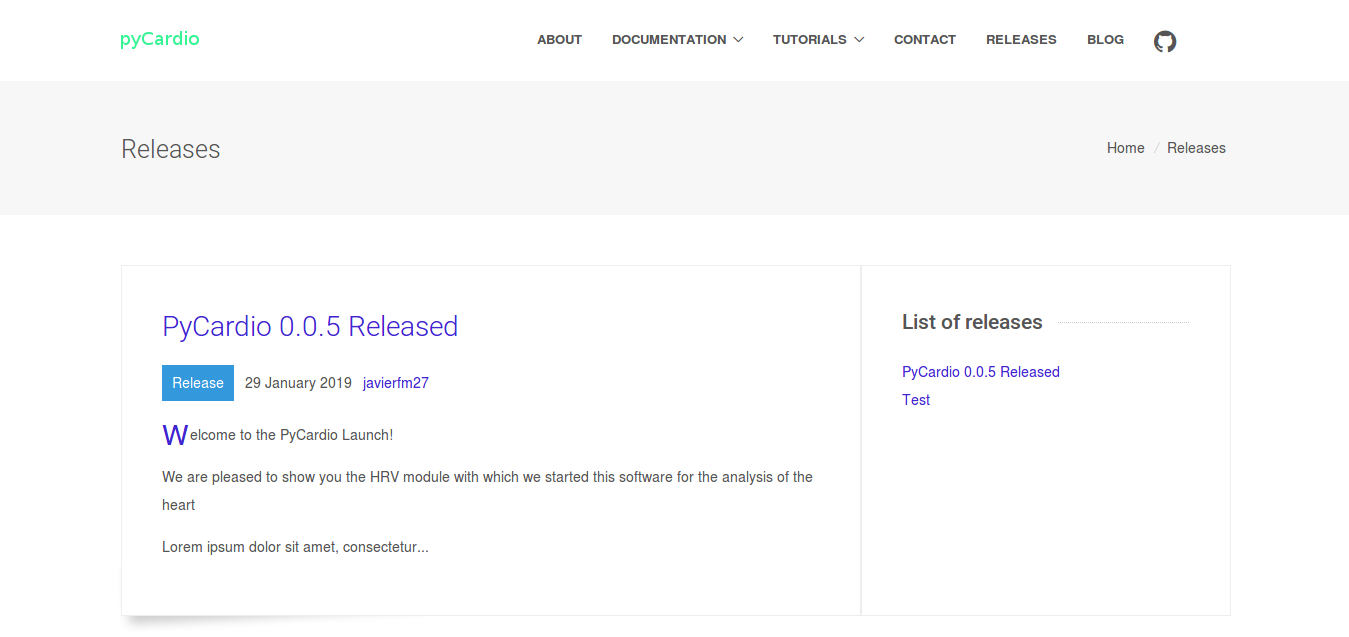
\includegraphics[width=0.5\textwidth]{img/release.png}
        \label{fig:releaseWeb1}
    }
    \subfloat[Captura de Release 2]{
        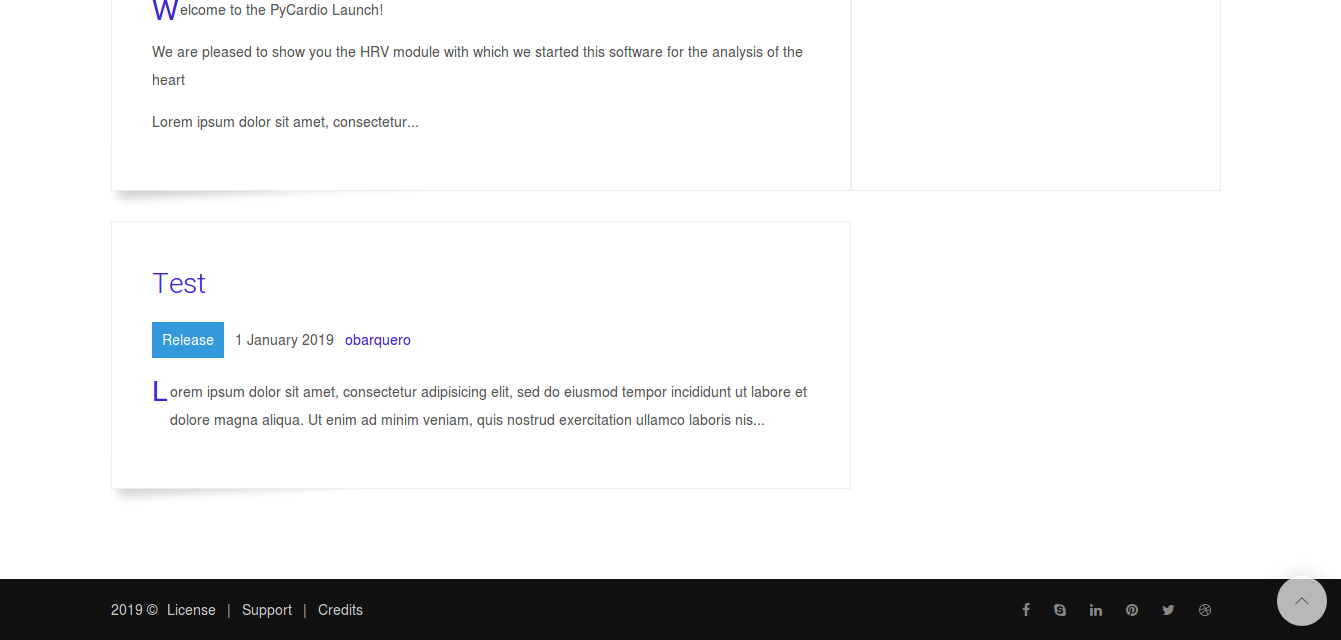
\includegraphics[width=0.5\textwidth]{img/release1.png}
        \label{fig:releaseWeb2}
    }
    \caption{Sección Release de la Web}
    \label{fig:releaseWeb}
\end{figure}

Para la implementación de esta parte se introduce por primera vez el uso de \textit{posts} del \textit{framework} \textit{Jekyll} comentado en la sección \ref{subsec:jekyll}. Es por esto, que para su desarrollo hacemos uso de dos \textit{layouts}, uno que se usará para el fichero \texttt{index.html} (el \textit{layout} utilizado es el mismo que anteriormente, \texttt{page.html}) de esta sección y otro \textit{layout} nuevo cuyo uso es para la escritura de los \textit{posts}, de forma que solo tengamos que preocuparnos de redactar en texto plano todo lo nuevo referente a la \textit{release} que estamos comentando. \\

El diseño del nuevo \textit{layout} se diseña con el objetivo de que cuando escribimos el \textit{post} se introduzca el autor, título y el contenido. Tanto el título como el contenido se darán a través del \textit{front matter}. La publicación que mostramos como ejemplo en el Listing \ref{code:release1} se corresponde al fichero \texttt{2019-01-29-0.0.5-pycardio-relesased.md}, siguiendo el convenio de nomenclatura que aconseja \textit{Jekyll}. \\


\begin{lstlisting}[caption=Ejemplo de publicación para la sección \textit{release},label={code:release1}]
  ---
layout: release
title: "PyCardio 0.0.5 Released"
author: "javierfm27"
category: [releases]
permalink: /:categories/:year/:month/:title
---
Welcome to the PyCardio Launch!


We are pleased to show you the HRV module with which we started this software for the analysis of the heart

Lorem ipsum dolor sit amet, consectetur adipisicing elit, sed do eiusmod tempor incididunt ut labore et dolore magna aliqua. Ut enim ad minim veniam, quis nostrud exercitation ullamco laboris nisi ut aliquip ex ea commodo consequat. Duis aute irure dolor in reprehenderit in voluptate velit esse cillum dolore eu fugiat nulla pariatur. Excepteur sint occaecat cupidatat non proident, sunt in culpa qui officia deserunt mollit anim id est laborum.

\end{lstlisting}

Si observamos el \textit{front matter} del ejemplo estamos catalogando nuestra publicación a la categoría de \textit{release}, esto lo hacemos debido a que en nuestra \textit{web} tendremos dos tipos de publicaciones: por un lado \textit{releases} y, por otro lado, las referentes al \textit{blog} de la \textit{web}. Por tanto, es una buena práctica diferenciarlas mediante categorías para su implementación por ejemplo a la hora de listar todas las publicaciones mediante la variable global \texttt{site.categories}.

\begin{figure}[H]
    \centering
    \subfloat[Ejemplo de Publicación 1]{
        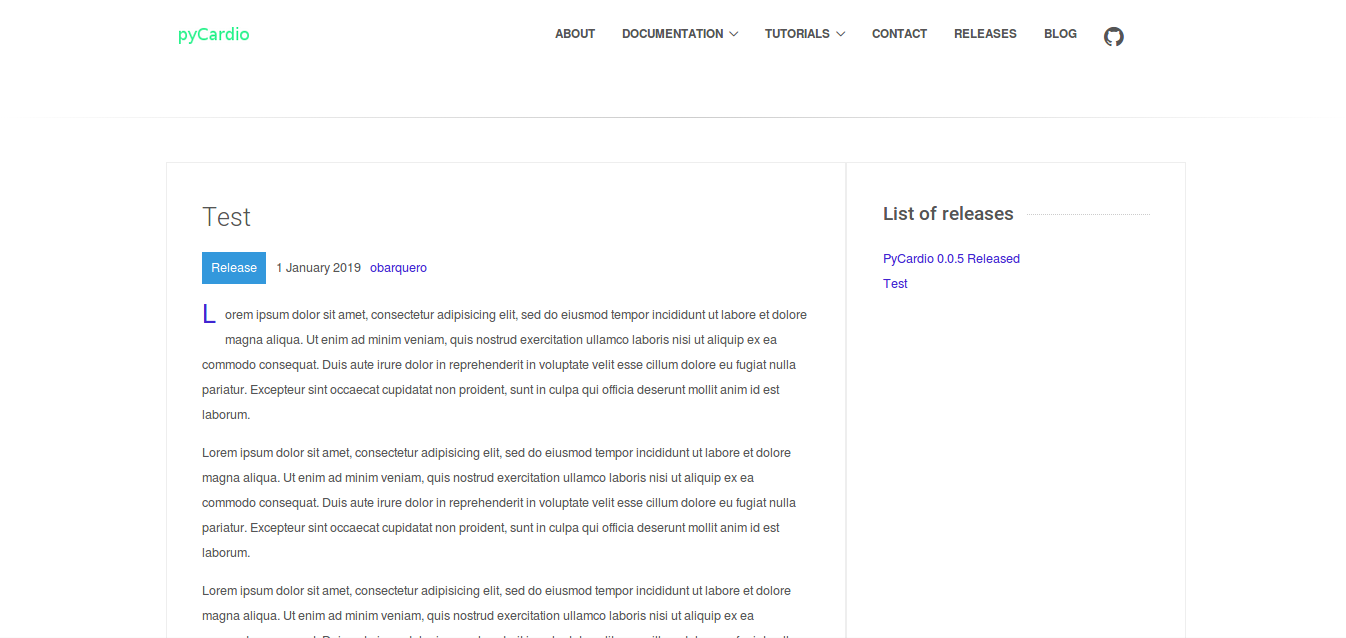
\includegraphics[width=0.5\textwidth]{img/only_release_1.png}
        \label{fig:onlyreleaseWeb1}
    }
    \subfloat[Ejemplo de Publicación 2]{
        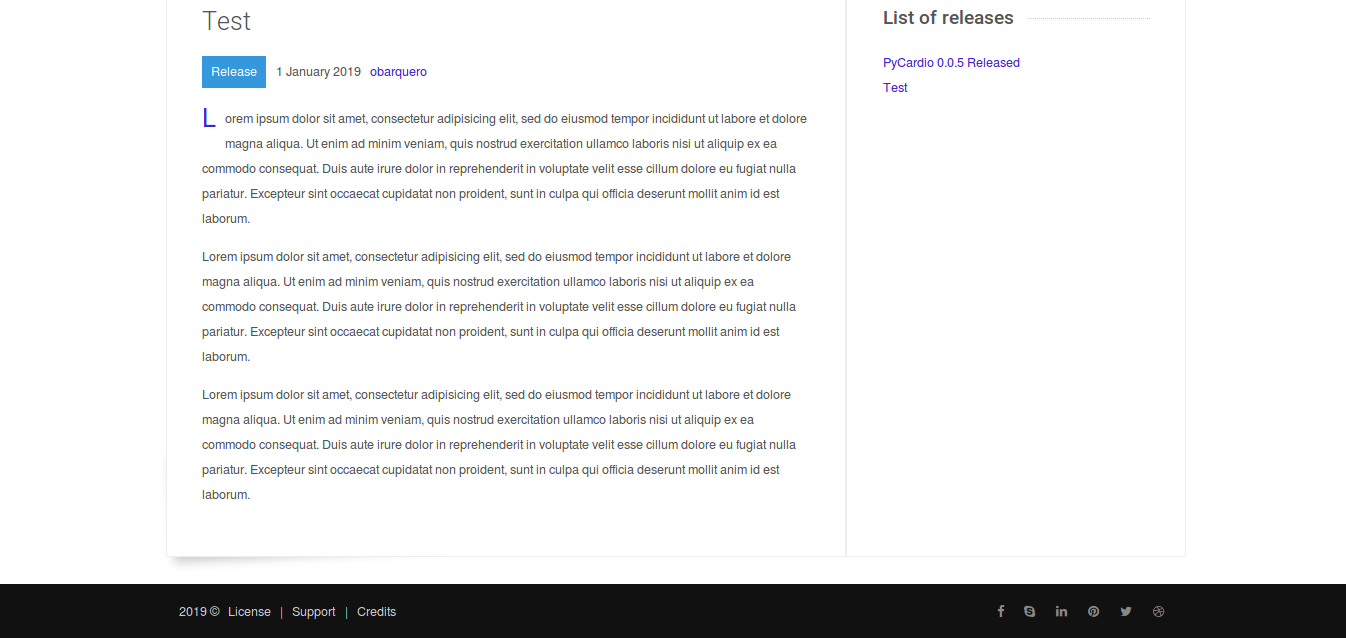
\includegraphics[width=0.5\textwidth]{img/only_release_2.png}
    }
    \caption{Aspecto Web de una publicación}
    \label{fig:onlyreleaseWeb}
\end{figure}

El resultado del Listing \ref{code:release1} es el mostrado por la figura \ref{fig:onlyreleaseWeb}. 

%%%%%%%%%%%%%%%%%%%%%%%%%%%%%%%%%%%%%%%%%%%%%%%%%%%%%%%%%%%%%%%%%%%%%%%%%%%%%%%%%%%%%%%%%%
%                       BLOG
%%%%%%%%%%%%%%%%%%%%%%%%%%%%%%%%%%%%%%%%%%%%%%%%%%%%%%%%%%%%%%%%%%%%%%%%%%%%%%%%%%%%%%%%%%

\section[Blog]{Blog \footnote{\url{https://javierfm27.github.io/blog/}}}
\label{sec:blogWeb}
Porción de la web centrada en mostrar todas las publicaciones que se escriben referente al \textit{software} de \textit{PyCardio} como nuevos usos que se han dado de este, noticias sobre su próximo lanzamiento, así como  publicaciones de los autores. Para su aspecto \textit{web} se ha seguido el mismo razonamiento de sencillez  de \ref{sec:releaseWeb} solo que, para esta sección, se ha cambiado el aspecto además de la adición de tres enlaces en el panel lateral. 

\begin{figure}[H]
    \centering
    \subfloat[Captura de Blog Web 1]{
        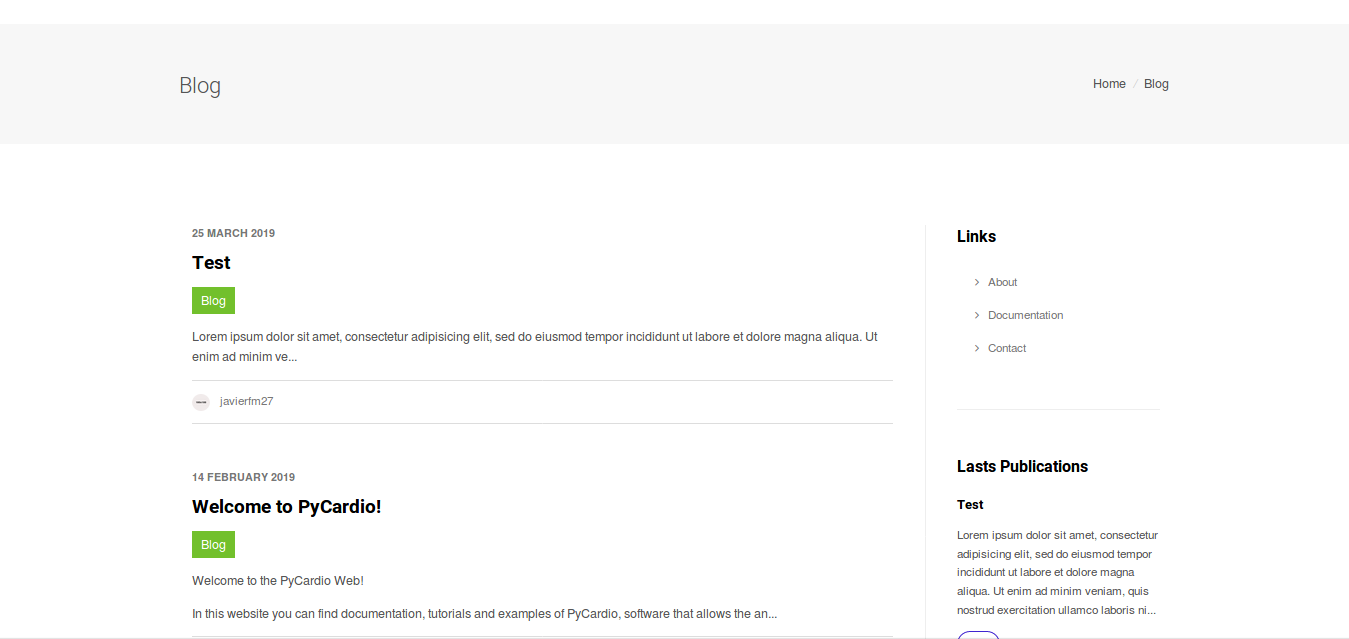
\includegraphics[width=0.5\textwidth]{img/blogWeb_1.png}
        \label{fig:blogWeb1}
    }
    \subfloat[Captura de Blog Web 2]{
        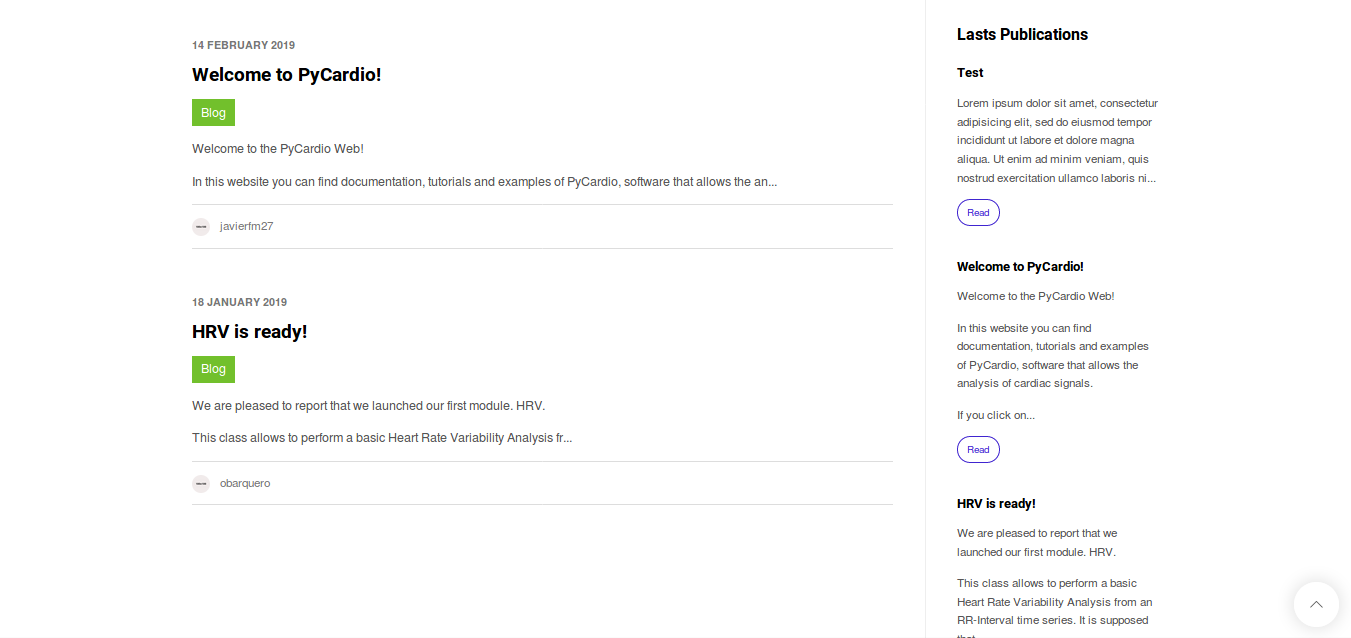
\includegraphics[width=0.5\textwidth]{img/blogWeb_2.png}
        \label{fig:blogWeb2}
    }
    \caption{Sección Blog de la Web}
    \label{fig:blogWeb}
\end{figure}

La implementación de esta parte sigue el procedimiento de la sección de \textit{release} donde distinguimos el fichero \texttt{index.html} de \texttt{/blog/} que usa el \textit{layout} de \texttt{page.html} y las publicaciones que se redactarán en texto plano que usarán uno nuevo denominado \texttt{blog.html}. Podemos distinguir en el código escrito en \ref{code:blogMD} cómo se asigna la categoría de \textit{blog}. El resultado de la publicación de la porción de código es el dado por \ref{fig:blogExample}.

\begin{figure}[h!]
    \centering
    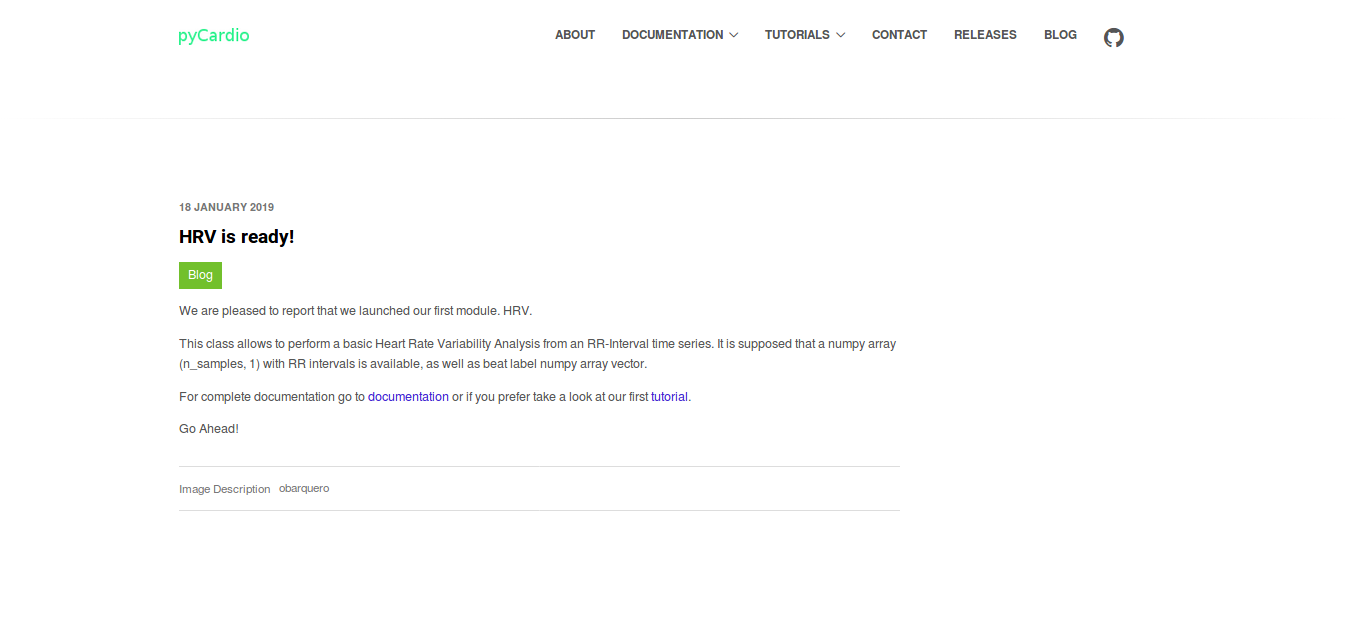
\includegraphics[width=\textwidth]{img/blog_example.png}
    \caption{Ejemplo de publicación para la sección de Blog}
    \label{fig:blogExample}
\end{figure}